\documentclass[12pt,a4paper,openright,twoside]{book}
\usepackage[utf8]{inputenc}
\usepackage{disi-thesis}
\usepackage{code-lstlistings}
\usepackage{notes}
\usepackage{shortcuts}
\usepackage{acronym}

\school{\unibo}
\programme{Corso di Laurea in Ingegneria e Scienze Informatiche}
\title{Integrazione di RAG e LLM nello Sviluppo del Software}
\author{Bollini Simone}
\date{\today}
\subject{Programmazione ad oggetti}
\supervisor{Prof. Viroli Mirko}
\cosupervisor{Dott. Aguzzi Gianluca}
\morecosupervisor{Dott. Farabegoli Nicolas}
\session{IV}
\academicyear{2023-2024}

% Definition of acronyms
\acrodef{RAG}{Retrieval-Augmented Generation}
\acrodef{AI}{Artificial intelligence}
\acrodef{LLM}{Large Language Model}


\mainlinespacing{1.241} % line spacing in mainmatter, comment to default (1)

\begin{document}

\frontmatter\frontispiece

\begin{abstract}	
I \ac{LLM} addestrati per sviluppare il codice sono oggi altamente efficaci e in grado di generare soluzioni utili e funzionanti.
L'addestramento fatto dai modelli è però su fonti e soluzioni generali, questo non da quindi la possibilità al modello di proppore soluzioni su misura per una specifica richiesta utilizzando casistiche già create dal programmatore o dalla propria azienda per casi simili. Da questo nasce l'esigenza di addestrare il modello per personalizzare le soluzioni proposte, contestualizzandole alla propria realtà aziendale e al proprio stile nel programmare.
Il \ac{LLM} non conosce le librerie interne dell'azienda, i pattern di programmazione adottati e quindi le risposte ottenute sono troppo generiche.
Per rispondere a questa esigenza entra in gioco la \ac{RAG} ovvero il processo di ottimizzazione dell'output di un \ac{LLM}, per permettergli di fruire una base di conoscenza personalizza, unica e privata, questa \textbf{matrice di conoscenza}  si inserisce tra quanto già appreso dal modello dai dataset utilizzati in fase di addestramento, estendendo la base dati sulla quale generare l'output con la risposta.
Questa tesi sperimenta l'integrazione di un \ac{RAG} con un \ac{LLM} per ottenere dal modello risposte personalizzate con conoscenze private e specifiche fornite da un dataset personalizzato.




\end{abstract}

\begin{dedication}
A Giulia persona eccezionale che ha cambiato in meglio la mia vita.
\newline Ai miei figli, il dono più grande di questo mondo.
\newline A tutta la mia famiglia sulla quale posso sempre contare.
\newline Grazie a tutti voi.
\end{dedication}

%----------------------------------------------------------------------------------------
\tableofcontents   
\listoffigures     % (optional) comment if empty
\lstlistoflistings % (optional) comment if empty
%----------------------------------------------------------------------------------------

\mainmatter

%----------------------------------------------------------------------------------------
\chapter{Introduzione}
\label{chap:introduction}
%----------------------------------------------------------------------------------------

\section{Essere programmatori nel 2025}
Sono disponibili tantissimi (IDE) per lo sviluppo del codice uno di questi è \textbf{Visual Studio Code}, mentre \textbf{Github} può essere lo strumento utilizzato per contenere e condividere progetti per lavore in maniera collaborativa. Può anche essere molto utile, \textbf{COLAB} che permette di eseguire in remoto codice che richiede molta memoria su GPU spesso non disponbili localmente.
Questi esempi mostrano una panoramica vasta e complessa, con un frequente cambio di software per realizzare un programma, modifiche fatte localmente su Visual Studio Code vengono trasferite su GitHub e poi riprese su Colab dove a sua volta vengono eseguiti Commit e Push sul progetto radice presente su GitHub.
La cosa che accomuna questi strumenti oggi è che dispongono tutti di assistenti di programmazione basati sull'intelligenza artificiale, in grado di completare il codice, suggerire correzioni e creare documentazione pertinente.
Lo schema di lavoro appenda descritto è stato da me attuato per realizzare questa tesi, ho utilizzato Visual Studio Code per scrivere il codice Pyhon, GitHub per condividere il progetto e Colab per eseguire la maggior parte del codice.
Una delle funzionalità offerte da questi assistenti è la la funzione di \textbf{Github Copilot} 'Generate Commit Message with Copilot' che propone il testo da utilizzare come descrizione di un commit, ho provato a riscontrare quanto fosse contestualizzato e coerente 
con quanto aggiornato e ho ottenuto il seguente risultato:
\begin{figure}[h]
    \centering
    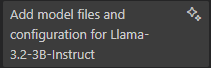
\includegraphics[width=0.5\linewidth]{figures/commit.png}
    \label{fig:enter-label}
\end{figure}
\newline
Ho trovato coerente e giusto quanto proposto ed eseguito il Commit.
Quanto è riuscito a fare Copilot è strabiliante, in pochi istanti ha analizzato il contesto dando come output una risposta semplice ma coerente rispetto a quanto cambiato.
L'uso di questi strumenti rende il lavoro molto più dinamico e permette di ridurre le interruzioni per cercare una soluzione o per trovare le giuste parole per descrivere
quanto fatto.
\begin{figure}[h]
    \centering
    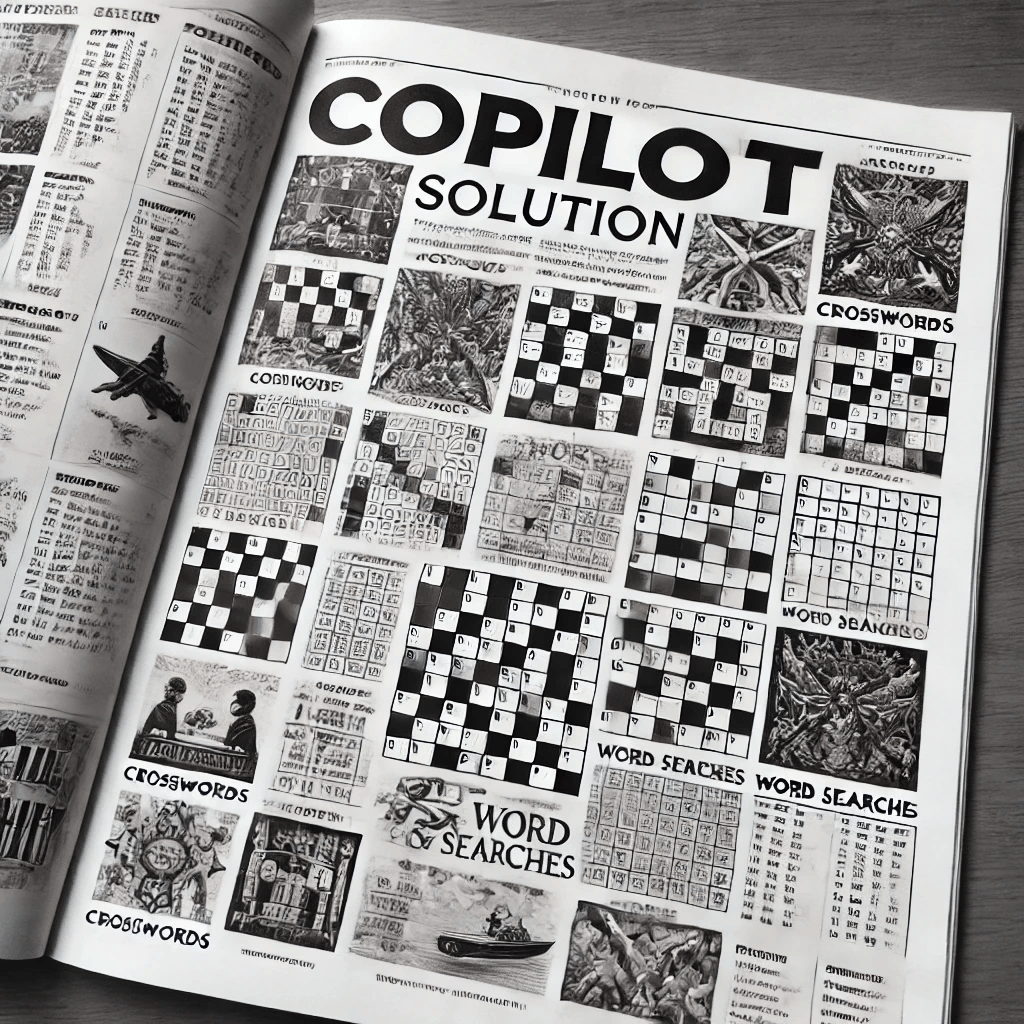
\includegraphics[width=0.5\linewidth]{figures/copilotsolutionSettimanaEnigmistica.png}
    \label{fig:enter-label}
\end{figure}
\newline
L'intelligenza artificiale sta rivoluzionando il modo in cui il software viene sviluppato, dando la possibilità a strumenti come Copilot di esplodere tutto il loro potenziale permettono di creare la spina dorsale di un progetto lasciando al programmatore il compito di verificare e correggere solo in parte il codice perché indirizzati e condizionati da quanto proposto. 
In progetti complessi questo non riduce il ruolo del programmatore, anzi lo eleva a compiti più precisi e complessi lasciando la stesura di parti del codice semplici e ripetitive al software stesso.
Sapere cosa chiedere e formulare correttamente le domande al LLM è fondamentale, esplicitando nel dettaglio con parole chiave mirate come deve essere realizzato il codice.
Altro compito complesso per il programmatore è non farsi troppo ammaliare dalle soluzioni proposte perché non sempre necessarie per quanto richiesto oppure diversa da quanto già conosciuto per realizzare una determinata funzione.
Questo nuovo modo di lavorare per mette di conoscere nuove soluzioni ma comporta test e tempo non sempre disponibile.
Il programmatore deve avere il controllo del progetto accettando generazione del codice automatica solo dove consapevole di quanto proposto e del suo impatto anche in casi di revisione e manutenzione futuri.
L'ultimo miglio da percorrere è la personalizzazione delle risposte del LLM, per ottenere risposte coerenti con quanto già realizzato e conosciuto, per fare questo entra in gioco la RAG.
\chapter{Addestrare un LLM per la Generazione del Codice}

L'addestramento di LLM per la generazione di codice di programmazione richiede una serie di passaggi metodici e risorse computazionali significative.
Conoscere questo processo è utile per la successiva integrazione con la RAG.
La procedura si divide nelle selle seguenti fasi:

\section{Raccolta e Preparazione dei Dati}

La qualità e la quantità dei dati di addestramento è di primaria importanza per addestrare il modello in maniera efficacie.
Per prepare un modello alla generazione di codice è essenziale utilizzare per il training codice sorgente proveniente da progetti reali, documentazione tecnica e esempi di codice ben strutturati.
Fonti comuni includono repository open source, piattaforme di condivisione del codice e documentazione tecnica che al momento è possibile trovare in grandi quantità su internet.
I dati raccolti devono essere puliti e pre-processati per rimuovere errori e informazioni non pertinenti, garantendo così un dataset di alta qualità per l'addestramento.

\section{Pre-Addestramento}
Il pre-addestramento è la fase in cui il modello apprende le strutture sintattiche e semantiche del linguaggio naturale e del codice. Durante questa fase, il modello viene esposto a grandi quantità di testo e codice, permettendogli di comprendere le regole grammaticali, i pattern comuni e le dipendenze contestuali. Questo processo utilizza tecniche di apprendimento non supervisionato, in cui il modello impara a prevedere la parola o il token successivo in una sequenza, sviluppando una comprensione approfondita delle strutture linguistiche.

\section{Fine-Tuning}
Dopo il pre-addestramento, il modello viene sottoposto a una fase di fine-tuning utilizzando dataset specifici del dominio, in questo caso, codice di programmazione. Il fine-tuning consente al modello di specializzarsi in compiti particolari, migliorando la sua capacità di generare codice coerente e funzionale. Questa fase può includere l'uso di tecniche di apprendimento supervisionato, dove il modello viene addestrato su coppie di input-output, come descrizioni di funzionalità e il relativo codice implementativo.

\subsection{Dataset per il Fine-Tuning}
\begin{itemize}
    \item \textbf{Descrizioni di Funzionalità}: Testi descrittivi che spiegano cosa dovrebbe fare il codice.
    \item \textbf{Codice Implementativo}: Esempi di codice che realizzano le funzionalità descritte.
\end{itemize}

\subsection{Tecniche di Fine-Tuning}
\begin{itemize}
    \item \textbf{Apprendimento Supervisionato}: Utilizzo di coppie input-output per addestrare il modello.
    \item \textbf{Apprendimento per Rinforzo}: Utilizzo di feedback per migliorare le prestazioni del modello.
\end{itemize}

\section{Architettura del Modello}
Gli LLM utilizzano tipicamente architetture basate su trasformatori, che sono particolarmente efficaci nell'elaborazione di sequenze di dati, come il testo e il codice. I trasformatori utilizzano meccanismi di auto-attenzione per valutare l'importanza di diversi elementi in una sequenza, permettendo al modello di comprendere le relazioni a lungo raggio tra parole o token. Questa capacità è cruciale per la generazione di codice, dove le dipendenze tra variabili e funzioni possono estendersi su intere porzioni di codice.

\subsection{Componenti Principali dei Trasformatori}
\begin{itemize}
    \item \textbf{Encoder}: Codifica l'input in una rappresentazione interna.
    \item \textbf{Decoder}: Genera l'output basandosi sulla rappresentazione interna.
    \item \textbf{Meccanismo di Attenzione}: Valuta l'importanza di diversi elementi in una sequenza.
\end{itemize}

\subsection{Varianti di Trasformatori}
\begin{itemize}
    \item \textbf{Trasformatori Autoregressivi}: Utilizzati per la generazione di testo (es. GPT).
    \item \textbf{Trasformatori Encoder-Decoder}: Utilizzati per compiti di traduzione e sintesi (es. BERT).
\end{itemize}

\section{Valutazione e Ottimizzazione}
Una volta addestrato, il modello deve essere rigorosamente valutato utilizzando metriche specifiche per la generazione di codice, come la correttezza sintattica, la funzionalità e l'efficienza del codice prodotto. I risultati della valutazione guidano ulteriori ottimizzazioni, che possono includere aggiustamenti dei pesi del modello, modifiche all'architettura o l'inclusione di dati di addestramento aggiuntivi per affrontare eventuali carenze.

\subsection{Metriche di Valutazione}
\begin{itemize}
    \item \textbf{Correttezza Sintattica}: Verifica che il codice generato sia sintatticamente corretto.
    \item \textbf{Funzionalità}: Verifica che il codice generato realizzi la funzionalità desiderata.
    \item \textbf{Efficienza}: Valuta le prestazioni del codice in termini di tempo di esecuzione e utilizzo delle risorse.
\end{itemize}

\subsection{Tecniche di Ottimizzazione}
\begin{itemize}
    \item \textbf{Aggiustamento dei Pesi}: Modifica dei pesi del modello per migliorare le prestazioni.
    \item \textbf{Modifiche all'Architettura}: Introduzione di nuove componenti o modifiche a quelle esistenti.
    \item \textbf{Integrazione di Dati Aggiuntivi}: Utilizzo di ulteriori dati di addestramento per migliorare le prestazioni.
\end{itemize}

\chapter{RAG}
Il termine RAG è l'abbrevazione del termine \textbf{Retrieval-Augmented Generation} \cref{fig:jumpstart-fm-rag.jpg} è un sistema che permette di estendere un modello di generazione del linguaggio con un modello di recupero, per ottenere risposte più coerenti e contestualizzate.
Allo scopo di:
\begin{itemize}
    \item migliorare la generazione di codice specifico per il proprio dominio e riducendo le allucinazioni;
    \item aumenta il contesto della domanda fatta al LLM;
    \item facilitare il debugging di sistemi complessi;
    \item supportare la creazione di documentazione aggiornata;
    \item permettere all'interno di un Team di migliorare la coerenza del codice scritto da diversi programmatori, per realizzare naturalmente senza forzature, codice più moderno utilizzando librerie e standard comuni.
\end{itemize}


\begin{figure}
    \centering
    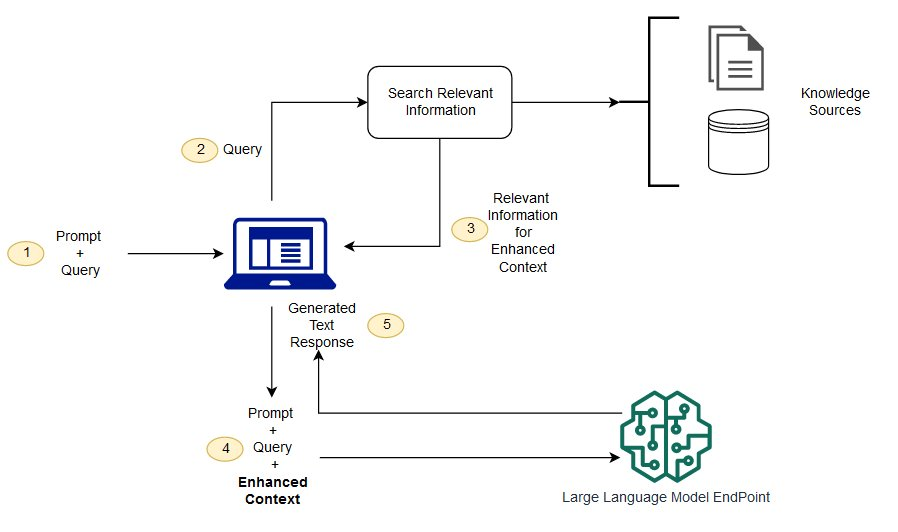
\includegraphics[width=.8\linewidth]{figures/jumpstart-fm-rag.jpg}
    \caption{Flusso concettuale dell'utilizzo di RAG con LLM}
    \label{fig:jumpstart-fm-rag.jpg}
\end{figure}


\chapter{Addestrare un LLM su dati custom(RAG)}
Per addestrare un LLM su dati custom per l'utilizzo con RAG, è necessario eseguire una serie di passaggi specifici per garantire la coerenza e la pertinenza delle risposte generate. Questi passaggi includono:


nsloth permette di addestrare in maniera efficente il modello

\begin{lstlisting}
from unsloth import FastLanguageModel
import torch
max_seq_length = 2048 # Choose any! We auto support RoPE Scaling internally!
dtype = None # None for auto detection. Float16 for Tesla T4, V100, Bfloat16 for Ampere+
load_in_4bit = False # Impostare a True per ridurre i pesi a 4bit quantizzandoli per ridurre uso di memoria, visto che il modello e' piccolo lascio Float16. 

model, tokenizer = FastLanguageModel.from_pretrained(
    model_name = "unsloth/Llama-3.2-3B-Instruct", # or choose "unsloth/Llama-3.2-1B-Instruct"
    max_seq_length = max_seq_length,
    dtype = dtype,
    load_in_4bit = load_in_4bit,
    # token = "hf_...", # use one if using gated models like meta-llama/Llama-2-7b-hf
)
\end{lstlisting}

\section{LORA}
LoRA (Low-Rank Adaptation of Large Language Models)
è una tecnica di allenamento popolare e leggera che riduce significativamente il numero di parametri allenabili. Funziona inserendo un numero inferiore di nuovi pesi nel modello e solo questi sono addestrati. Ciò rende l'allenamento con LoRA molto più veloce, efficiente in termini di memoria e produce pesi modello più piccoli (alcune centinaia di MB), che sono più facili da archiviare e condividere.

\begin{lstlisting}
    model = FastLanguageModel.get_peft_model(
    model,
    r = 16, # Choose any number > 0 ! Suggested 8, 16, 32, 64, 128
    target_modules = ["q_proj", "k_proj", "v_proj", "o_proj",
                      "gate_proj", "up_proj", "down_proj",],
    lora_alpha = 16,
    lora_dropout = 0, # Supports any, but = 0 is optimized
    bias = "none",    # Supports any, but = "none" is optimized
    # [NEW] "unsloth" uses 30% less VRAM, fits 2x larger batch sizes!
    use_gradient_checkpointing = "unsloth", # True or "unsloth" for very long context
    random_state = 3407,
    use_rslora = False,  # We support rank stabilized LoRA
    loftq_config = None, # And LoftQ
)
\end{lstlisting}

\section{Modello PreTreinato}
Il modello ha già una conoscenza di base generica.
\begin{lstlisting}
from unsloth.chat_templates import get_chat_template

tokenizer = get_chat_template(
    tokenizer,
    chat_template = "llama-3.1",
)
FastLanguageModel.for_inference(model) # Enable native 2x faster inference

messages = [
    {"role": "user", "content": "parlami del mare Adriatico"},
]
inputs = tokenizer.apply_chat_template(
    messages,
    tokenize = True,
    add_generation_prompt = True, # Must add for generation
    return_tensors = "pt",
).to("cuda")

from transformers import TextStreamer
text_streamer = TextStreamer(tokenizer, skip_prompt = True)
_ = model.generate(input_ids = inputs, streamer = text_streamer, max_new_tokens = 128,
                   use_cache = True, temperature = 1.5, min_p = 0.1)
\end{lstlisting}

\section{Preparazione Dataset}

\section{Addestramento del modello}
Usando SFTTrainer
\section{FOrmatazione con i TAG di lamas}
\begin{lstlisting}
from unsloth.chat_templates import train_on_responses_only
trainer = train_on_responses_only(
    trainer,
    instruction_part = "<|start_header_id|>user<|end_header_id|>\n\n",
    response_part = "<|start_header_id|>assistant<|end_header_id|>\n\n",
)
\end{lstlisting}
\section{Addestramento vero e proprio}
\begin{lstlisting}
trainer_stats = trainer.train()
\end{lstlisting}
Possiamo vedere la Training Loss
il livello di errore, sposta i pesi imparando dal modello
nel mio caso la loss diventa 
\section{Sfida top LLM}
 Per la codifica, le persone stanno persino confrontando le sue prestazioni con il Claude-3.5-Sonet di Anthropic, che può ancora essere considerato il migliore. Per lo più le persone concludono che Sonnet è ancora il re della programmazione, ma come guidatore quotidiano, il modello di DeepSeek è un sostituto generale di GPT-4o. È grande però se vuoi auto-ospitarti: ha 671 miliardi di parametri addestrabili, che richiedono una quantità minima di 380 GB di memoria GPU.

\section{Parsing}
Inizialmente, il sistema analizza la Knowledge Base e ne estrae le informazioni in modo strutturato. Questo processo pu\`o includere:
\begin{itemize}
    \item Analisi di documenti come PDF, Word, Excel o pagine HTML.
    \item Estrazione di informazioni da immagini o tabelle.
\end{itemize}

\section{Captioning}
Per arricchire ulteriormente il contesto, i RAG possono utilizzare tecniche di captioning per generare descrizioni testuali delle immagini presenti nella Knowledge Base. Queste descrizioni vengono poi integrate con le informazioni estratte dal parsing.

\section{Splitting}
Le informazioni testuali estratte vengono suddivise in \textit{chunks} di dimensioni appropriate per il modello linguistico. Questa fase \`e cruciale per garantire un'elaborazione efficiente, tenendo conto dei limiti di memoria e di capacit\`a computazionale.

\section{Vettorizzazione}
Ogni \textit{chunk} di testo viene trasformato in un vettore numerico che rappresenta il significato semantico del testo stesso. Questi vettori sono memorizzati in un database vettoriale, che consente ricerche semantiche rapide ed efficienti.

\section{Interrogazione e Recupero}
Quando un utente pone una domanda al sistema, questa viene trasformata in un vettore numerico. Il sistema ricerca quindi i vettori pi\`u simili nel database vettoriale, identificando i \textit{chunks} di testo pi\`u pertinenti.

\section{Generazione della Risposta}
I \textit{chunks} di testo recuperati vengono forniti come contesto al modello linguistico generativo, che genera una risposta coerente e completa, basandosi sia sulla propria conoscenza generale sia sulle informazioni specifiche recuperate.

\chapter{Vantaggi e Sfide dei RAG}

\section{Vantaggi}
L'utilizzo dei RAG offre numerosi vantaggi:
\begin{itemize}
    \item \textbf{Maggiore accuratezza e pertinenza delle risposte:} I RAG consentono di fornire risposte pi\`u precise e contestualizzate grazie all'integrazione di informazioni specifiche del dominio.
    \item \textbf{Riduzione delle allucinazioni:} L'utilizzo di una Knowledge Base affidabile aiuta a limitare la generazione di informazioni false o inventate.
    \item \textbf{Possibilit\`a di personalizzazione:} I RAG possono essere adattati a specifiche esigenze di dominio o aziendali.
\end{itemize}

\section{Sfide}
Nonostante i vantaggi, l'implementazione dei RAG presenta alcune difficolt\`a:
\begin{itemize}
    \item \textbf{Complessit\`a di sviluppo:} La creazione di un sistema RAG efficiente richiede competenze avanzate di software engineering e intelligenza artificiale.
    \item \textbf{Gestione della Knowledge Base:} La Knowledge Base deve essere accuratamente selezionata, strutturata e mantenuta aggiornata.
    \item \textbf{Valutazione delle performance:} Richiede la creazione di dataset di test specifici e l'intervento di esperti di dominio.
\end{itemize}


\chapter{Conclusione}
Il 6 novembre 2024 Donal Trump ha vinto per la seconda volta le elezioni Americane, sentendo questo annuncio ho subito ripensato ai fatti di Capitol Hill, del 6 gennaio 2021 e quel giorno non avrei mai immaginato che sarebbe tornato ad essere presidente degli Stati Uniti. Con questa introduzione non voglio addentrarmi in nessun discorso politico, vorrei solo sottolineare lo stupore provato per questo recente episodio ma incredibilmente  non è nulla per me rispetto a quanto l'AI mi sorprende ogni giorno di più, da quando ho provato per la prima volta strumenti come ChatGPT, NotebookLM e Github Copilot (per citarne solo alcuni).
In questa Tesi nel cercare di documentarmi ho osservato interessato i cambiamenti e gli sviluppi dell'AI da ottobre 2024 a Gennaio 2025 è stato per me qualcosa di incredibile, una sfida continua tra i massimo attori e programmatori del mondo nel fornire il modello o lo strumento di supporto più entusiasmante e funzionale.
Per questa tecnologia siamo in un era fantastica dove è facile reperire documentazione e preziosissimo codice OpenSorce (escluso il modello stesso :-!).
Chiedendo alle persone a me vicine il loro punto di vista su gli sviluppi e scenari di crescita che porterà in tutti i settori questa nuova tecnologia è un senso di paura per la sparizione di tanti lavori e un dominio sempre maggiore della macchina sull'uomo. 
Non ho la minima idea di come sarà il mondo tra vent'anni, alcuni dicono sempre lo stesso, qualche moda e tecnologia diversa ma l'uomo è sempre lo stesso nel bene o nel male.
Ma per me questa tecnologia è paurosamente incredibile, alza l'asticella e la velocità di sviluppo in qualsiasi fronte in maniera immaginabile. In Matrix ricordo gli addestramenti di Neo in pochi istanti nell'imparare arti marziali o nel guidare un aereo, questi strumenti sembrano avere questo potere, hanno la possibilità di elaborare, comprendere e generare qualsiasi cosa in un istante.
Spero con tutto il cuore che la realtà non rispecchi quanto visto nei film di fantascienza,
scrivere questa tesi mi ha molto destabilizzato addentrandomi nel mio piccolo nella potenza di questi strumenti.
Senza dimenticare di avere in mano strumenti "openSource", mi chiedo quale è già oggi il massimo livello reale di sviluppo di queste tecnologie.




\lstinputlisting[float,language=Java,label={lst:random-code}]{listings/HelloWorld.java}


%----------------------------------------------------------------------------------------
% BIBLIOGRAPHY
%----------------------------------------------------------------------------------------

\backmatter

\nocite{*} % Remove this as soon as you have the first citation

\bibliographystyle{alpha}
\bibliography{bibliography}

\end{document}
